\section {Introduction}
%\begin{quote}
%Draw the reader in--Why should I read this?
%Cite at least 3 previous studies--What has been done already?
%Establish the `research gap'--What hasn’t been done?
%Brief overview of study--What is the purpose of your study?
%\end{quote}


\subsection {What's the problem?}
Members of the Church of Jesus Christ of Latter-day Saints are admonished to study from general conference talks. The LDS General Conference Corpus, hereafter referred \emph{LDS-GCC} increases bi-annually. Many members have access to search tools and a topical index of scriptures, but no topical index exists for talks. The ability to navigate through talks in a new way could help laymembers to more easily make connections. The need for such tools increases over time since the amount of information increases. 

\subsection{Existing Tools}
Various websites exist for LDS members to use, but the capabilities they provide could be enhanced. Two main sites are http://www.lds.org and http://scriptures.byu.edu; they are are updated often. http://www.lds.org seems to focus on globalization and media while http://scriptures.byu.edu focuses on providing a reverse citation technique. Normally, talks from the church cite scriptures at the end of the talk; http://scriptures.byu.edu uses those to link from scriptural passages to the talks rather than the other way around. The advantage is that if you want to learn more about a passage, you can look at whatever cites it. Both sites appear have a Lucene-like search functionality (McCandless et al 2010; Luke 2013), but search-based tasks are known to be problematic when a user is new to a subject area or is unfamiliar with the particular vernacular of a domain--a typical problem for newer members. \emph{The same problem applies to Mark Davies' interface}\footnote{Mark Davies, Ph.D., is a professor of BYU with an amazing amount of experience in corpus linguistics. His interface for corpora are well known for their speed, consistency, reliability, and representativeness.} to the corpus (http://www.lds-general-conference.org/), which is less a tool for studying talks in-depth and more a tool built to perform searches in the area of corpus linguistics.

\subsection{Why More Tools Are Needed}
The LDS church gains new members yearly, numbering in the thousands and the number of talks is increasing as well. Making it easier to navigate documents and therefore focus learning/teaching efforts could greatly aid both the erudite and the newcomer. Advanced recommendation systems could be used to alleviate this burden as well, which I leave to future work \footnote{Specifically, my thesis (in process) is an attempt at producing a recommendation system for \emph{LDS-GCC}.}. Although this work does not go so far as to produce a recommendation system, it does pave the way for that by demonstrating that Gibbs Sampling can be used to automatically identify and cluster related words into clusters interpreted as topics. These word clusters can then be labeled and people with access to the internet can peruse documents that are ranked along the dimension corresponding to a given topic. This system is a major improvement over relying on keyword-based searches to locate documents since sometimes a document doesn't mention a topic directly, in spite of being about the topic. An example of this is a talk on the `Word of Wisdom' before the revelation given to Joseph Smith, Jr. was referred to as such. In this paper, I will refer to this topical index as \emph{iTopTalk}. (Semi) automated  work related to this also include the work of Hilton III \shortcite{hilton-2008-intertext-abinadi} that performs plagiarism detection techniques to determine how words of scriptural characters are influenced linguistically by previous characters.\footnote{Note that www.LDS.org attempts to support topic-based searches (e.g. ``Talks on Faith''), but rather than searching by topic, this site's search simply performs the search in a restricted ``talks'' domain. The only way the site seems to allow users to search by topic is by year, so in order to find a list of all talks that are tagged as being about a topic (e.g. `Faith').}

\subsection{Brief Overview}
This project aims to produce an intuitive, easy-to-use topical index, \emph{iTopTalk}, for \emph{LDS-GCC}. As a result, any website that allows users to read LDS general conference talks should be able to use \emph{iTopTalk} as an topical index. The parameters of the the topic model are inferred via \emph{(Collapsed) Gibbs Sampling}
(Porteous et al. 2008), %\shortcite{Porteous:2008:FCG:1401890.1401960} 
 although \emph{Variation Inference} could be used as well (Blei et al. 2006). %\shortcite{blei2006variational}
%. We use Collapsed Gibbs sampling in this work. 
\emph{iTopTalk} is an LDA-based system, trained for general conference talks. Much work has been done in the area of topic modeling, but applying them to this dataset, at least for this purpose is novel.

\emph{iTopTalk} is a natural result of \emph{LDA} which is a topic model of topic probability and word-topic assignments. Although \emph{LDA} model does not include labels for topics, it does provide a list of key words for each topic from which a human who is familiar with the documents can manually assign labels. I will report the 10 most frequent LDA topics and the labels I assign to them. Furthermore, 10 main documents will be listed, showing that talks can be located via the topical content. A link to the system will also be supplied.


\section {Method}
%\begin{quote}
%Corpus--Describe the corpus/corpora that you are using (Option A) or the corpus that you are creating (Option B)
%Data analysis--How will you measure your findings?
%\end{quote}

\subsection{Corpus}
The \emph{LDS-GCC} consists of over 10,000 talks. Some were extemporaneously given while others were scripted. The intended audience is generally only either the male members of the church, female members of the church, or the entire church. The size and the extent of internationality of the audience is increasing over time. The LDS church currently has over 15 million members, with the majority living outside the United States of America. Talks have traditionally been given first in English, then are translated into other languages. In 2014, the church allowed speakers to speak in their native language instead. This work won't have to worry about the possible noise that that change would introduce since we use the older dataset that only goes up to October 2013 rather than to October 2014. 

I use the subset of the \emph{LDS-GCC} this is available online via www.lds.org combined with those talks that are already in the public domain\footnote{Talks from the Journal of Discourse are in the public domain.}. This is a subset of the documents used by Mark Davies in his interface to the corpus. The date of authorship for these talks are ranges of either 1846-1886 or 1942-2013. In total over 1,400 talks are in this subset. 

\subsection{Course Requirement}
The requirements of this project state that a corpus must be created or used. In the case of this work, both tasks were performed, but emphasis is on `Option A' which is to use a corpus. Since I had to obtain and clean the documents that were not already in the corpus, I also performed tasks associated with `Option B'l. 

\subsection{Data Gathering}
First, data is gathered. Then `noise' is filtered out. This mostly means removing HTML markup, removing punctuation, lower-casing every character, and using a stopword list. The mallet toolkit, an open source tool used here to perform Gibbs Sampling, comes with a decent stopword list. I augmented the default list with some religious high frequency words, including `jesus', `christ', `god', `gods'. These were discovered by trial and error as I ran and reran this process. Ideally, one would consult a frequency chart or a TF-IDF algorithm to more systematically select high-frequency words and perhaps replace the mallet stoplist entirely with a custom one.

\subsection{Processing}
Each (cleaned) document is fed into LDA as input. Gibbs Sampling, when used to infer an LDA model, must be provided 2 main parameters: \emph{K}, and a number of iterations. \emph{K} corresponds to the number of topics that the researcher believes to exist in the documents. If the number is too low, then some topics will be confounded with others (merged into another topic or split among more than 1 other topic)--i.e. they are `conflated'. Trial and error is also used here until a good number is found. I performed this task in previous work and found that 200 was a decent value for k. Generally, Gibbs Sampling needs at least 100 iterations to learn the word-topic assignments, but trial and error is often used. I found that 1000 iterations was sufficient and completed in under 10 minutes. 

In fulfillment of `Option A', I perform the following key tasks: 

\begin{itemize}
    \item use \emph{Collapsed Gibbs Sampling} to infer the parameters of an \emph{LDA} model,
    \item use the Mallet toolkit will be used to run collapsed Gibbs sampling,
    \item label 10 topics\footnote{Since labelling is a manual process, it can lead to some bias. Although this is the case, when the system is made publicly available online, I can rely on input from end-users when it comes to usefulness/correctness of labels. For now, I trust my instinct and that of my wife.},
    \item explore at least 10 documents which have one of the 10 as their main topic,
    \item provide a discussion on the \emph{LDS-GCC} of the algorithm, and
    \item write this report.
\end{itemize}

\subsection {Goal}
This study produces the following:
\begin{quote}
	${1}:$ Produce \emph{iTopTalk}, an \emph{LDA}-based index of topics for LDS General Conference talks and make it publicly available online.
    
	${2}:$ Produce and report a partially labelled set of topics and list 10 talks whose predominant topic is 1 if these 10 topics.
\end{quote}

\subsection{Evaluation}
The \emph{LDS-GCC} of LDA is sorted by frequency, then the 10 most common topics are then labelled. Finally, within each topic, talks are sorted based on the percentage of words tagged with the given topic. I will select 10 talks (1 from each topic) and show that the main topic assigned to them makes sense.  talk per topic will be reported here. 

\section{Results}
%\begin{quote}
%Appropriate visuals (Tables, Graphs, Figures)
%Appropriate quantitative results
%\end{quote}

First off, it is worth noting that \emph{iTopTalk} is now publicly available online at http://bean5.github.io/\emph{LDS-GCC}-talk-topics/TalkTopicIndex.html. The interface is still in beta, but the \emph{LDS-GCC} of \emph{iTopTalk} itself is ready for public use. Feel free to experience the system yourself.

Figure \ref{figure:topics_labels} contains the ten most common topics according to \emph{iTopTalk}. The figure also includes the frequency of those topics (out of 200 topics), the manually-assigned labels, 1 selected talk from each, the frequency of the topic within the selected talk, and the year the talk was given.

\begin{landscape}
    \begin{figure}[ht!]
        \centering
        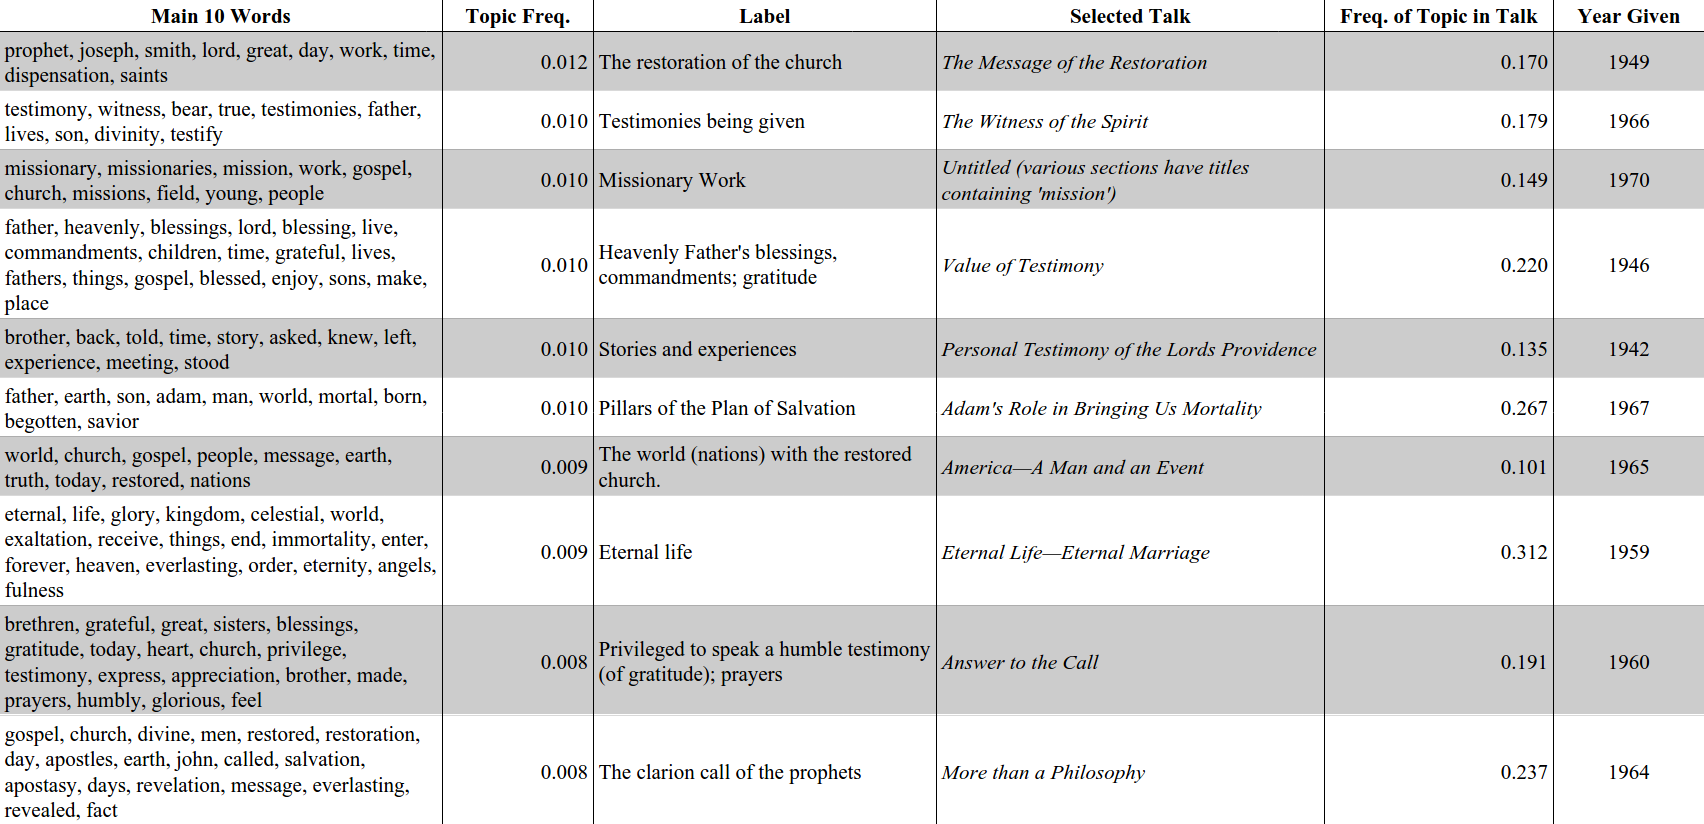
\includegraphics[width=230mm]{output.png}
        %\caption{Caption: Topics (words), metadata, and metadata of select talks.}
        \label{figure:topics_labels}
    \end{figure}

\end{landscape}

Just by glancing at the word clusters, it is apparent that Gibbs Sampling is finding clusters that are coherent. Because of this, it was easy to label the topics (being familiar with LDS talks helped, too). The titles of the talks that have one of these main topics are not surprising. Every one of the main topics had at least 1 document containing that devoted over 10\% of its words to the topic.

Interestingly, all the selected talks were published before 1971, which was fairly long ago. A possible reason why this might be the case is given later here.


\section{Discussion}

\subsection{Interpretation of Qualtitative Results}
Just from Figure \ref{figure:topics_labels}, we can draw various conclusions. 

One conclusion we could draw is that \emph{iTopTalk} works. One might argue that another system might work better, but that would require an in-depth comparison using evaluation metrics. Notwithstanding, \emph{iTopTalk} stands on its own. It can be used to locate talks that focus on a particular topic. 

\emph{iTopTalk} can provide quantitative measures such as frequency of topic and percentage of talk devoted to a given topic. This means that \emph{iTopTalk} can be used in quantitatively, just as Mark Davies' \emph{LDS-GCC} interface can be used. The difference is that \emph{iTopTalk} focuses on machine-learned topics while Mark Davies' interface is focuses on word-search--and any other feature known to his suite for corpora.

LDS talks published between 1940 and 1970 are likely to devote at least 10\% of their content to any one topic, given a common topic while talks outside that range were not as likely to rank as high. In previous work, I found that the entropy of general conference is increasing. It might very well be the case that talks are no longer focusing on one topic in more recent talks. This would explain why they are not high ranking within any 1 topic and would explain why entropy is increasing overall in conference over time. 

\subsection{Implications and limitations of findings}
\subsubsection{Implications}
Since \emph{iTopTalk}s, its \emph{LDS-GCC} can be integrated into websites that provide users with access to talks in the \emph{LDS-GCC}. It would probably be integrated as a topical index and might take on a form that is more interactive and intuitive than the current public interface. 

Because during the process of producing \emph{iTopTalk}, data was gathered such as topic distributions, we can apply a cosine similarity metric to produce a similar metric between talks. I intentionally leave this to future work (my thesis) due the the depth and degree to which it would not fit in a paper of this size.

\subsubsection{Limitations}
\emph{iTopTalk} is not a recommendation system at a talk-level and it has no search interface, although internet browsers typically provide a search+find feature that might allow a user to perform searches anyways. \emph{iTopTalk} is a recommendation system at the topic-level and required gathering of data, cleansing and normalization of data, and a parameter k. In related work, finding a way to automatically set k is desirable and various methods exist. Here, I took a manual trial-and-error approach, which is certainly a limitation.

\emph{iTopTalk} is already outdated. I intentionally only ran it on the talks up to 2013 because 2014 introduced talks not originally given in English. Of course, one might assume that those talks don't introduce too much noise, or one could circumvent the problem by not including those, but that would require investigation.

Stopwords were not systematically chose, but rather were chosen manually based on intuition only. Improving this part of the process could lead to less ambiguity in topics, less bias, and perhaps better results overall.

\emph{iTopTalk} was run on only the publicly available subset of \emph{LDS-GCC}. Naturally, it would be interesting to see how the system fairs if it were run on the entire \emph{LDS-GCC} dataset, but since some talks just aren't in the public domain and the LDS church prefers not to allow easy access to these, the reach and impact of such a system not have much more impact than this one due to fair use and copyright restrictions. 

\subsection{Summary of Full Study}
The \emph{LDS-GCC} is not outside the domain of automatically indexible corpora. A Latent Dirichlet Model, inferred via Gibbs Sampling, was successfully used to produce intelligible, coherent topics. This \emph{LDS-GCC} was easily labeled by hand and shows that further work in this area is possible. 